\documentclass{beamer}
\usepackage[spanish]{babel}
\usepackage[utf8]{inputenc}
\usepackage[nodayofweek,level]{datetime}
\usepackage{pgfpages}
\usepackage{hyperref}
\usepackage{minted}
\usepackage{hyperref}

\newcommand{\mydate}{\formatdate{10}{12}{2021}}

\usetheme{Madrid}
\title{Semánticas de lenguajes}
\subtitle{Especificación de un lenguaje imperativo con maude}
\author{Sergio García Sánchez}
\institute{UCM}
\date{\mydate}
\graphicspath{ {images/} }

\BeforeBeginEnvironment{minted}{\medskip}
\AfterEndEnvironment{minted}{\medskip}


\begin{document}

    \begin{frame}
        \titlepage
    \end{frame}

    \begin{frame}
        \frametitle{Indice}
        \tableofcontents
    \end{frame}


    \section{Introducción}
    \begin{frame}{Introducción}
        \begin{itemize}
            \item Especificación formal de un lenguaje imperativo
            \item Características del lenguaje
            \item Representación de la sintaxis
            \item Representación de la semántica mediante reglas de reescritura
            \item Ejecución la especificación
        \end{itemize}
    \end{frame}

    \section{Sintaxis}
    \begin{frame}[fragile]{Memoria}
        \begin{minted}[fontsize=\small]{haskell}
        sorts Pair Memory .
        subsort Pair < Memory .
    
        op [_,_] : Qid Int -> Pair [ctor] .
        op none : -> Memory [ctor] .
        op __ : Memory Memory -> Memory [ctor assoc comm id: none] .

        op _ [_\_] : Memory Qid Int -> Memory .
        eq ( M [ Q , V ]) [ Q \ V' ] = [ Q , V' ] M .
        eq M [ Q \ V ] = [ Q , V ] M  [owise] .
        
        op find : Memory Qid -> Int .
        eq find (M [Q, V] M', Q) = V .
        eq find (M, Q) = 0 [owise] .
        \end{minted}
    \end{frame}

    \begin{frame}[fragile]{Tipos}
        \begin{minted}[fontsize=\small]{haskell}
        sorts Type Index .
        subsorts Qid Int Index < Type .

        op _<_> : Type Type -> Index [ctor] .

        op load : Memory Type -> Type .
        eq load(M, Q) = find(M, Q) .
        eq load(M, I) = I .
        eq load(M, In) = find(M, toQid(In, M)) .
        \end{minted}
    \end{frame}

    \begin{frame}[fragile]{Expresiones}
        \begin{minted}[fontsize=\small]{haskell}
sort Expression .
subsort Type < Expression .
        
op _sum_ : Expression Expression -> Expression [ctor assoc comm] .
op _less_ : Expression Expression -> Expression [ctor] .
op _mult_ : Expression Expression -> Expression [ctor assoc comm] .

op eval : Expression Memory -> Type .
eq eval (T sum T', M) = load(M,T) + load(M,T') .
eq eval (T less T', M) = load(M,T) - load(M,T') .
eq eval (T mult T', M) = load(M,T) * load(M,T') .
eq eval (T, M) = load(M, T) [owise] .
        \end{minted}
    \end{frame}

    \begin{frame}[fragile]{Condiciones}
        \begin{minted}[fontsize=\small]{haskell}
sorts Condition MultipleCondition .
subsort MultipleCondition < Condition .
        
op _eq_ : Expression Expression -> Condition [ctor] .
op _neq_ : Expression Expression -> Condition [ctor] .
op _gt_ : Expression Expression -> Condition [ctor] .
op _gte_ : Expression Expression -> Condition [ctor] .
op _lt_ : Expression Expression -> Condition [ctor] .
op _lte_ : Expression Expression -> Condition [ctor] .
        
op _&&_ : Condition Condition -> MultipleCondition [ctor assoc comm] .
op _||_ : Condition Condition -> MultipleCondition [ctor assoc comm] .
        \end{minted}
    \end{frame}

    \begin{frame}[fragile]{Condiciones}
        \begin{minted}[fontsize=\small]{haskell}
op eval : Condition Memory -> Bool .
eq eval(E eq E', M) = load(M, eval(E, M)) == load(M, eval(E', M)) .
eq eval(E neq E', M) = load(M, eval(E, M)) =/= load(M, eval(E', M)) .
eq eval(E gt E', M) = load(M, eval(E, M)) > load(M, eval(E', M)) .
eq eval(E gte E', M) = load(M, eval(E, M)) >= load(M, eval(E', M)) .
eq eval(E lt E', M) = load(M, eval(E, M)) < load(M, eval(E', M)) .
eq eval(E lte E', M) = load(M, eval(E, M)) <= load(M, eval(E', M)) .
            
eq eval(C && C', M) = eval(C, M) and eval(C', M) .
eq eval(C || C', M) = eval(C, M) or eval(C', M) .
        \end{minted}
    \end{frame}

    \begin{frame}[fragile]{Asignaciones}
        \begin{minted}[fontsize=\small]{haskell}
sort Assig .
 
op _=_ : Type Expression -> Assig [ctor] .
op [ _ < _ > < _ > ] = _ : Qid Type Type Expression -> Assig [ctor] .
op _=[_] : Type Array -> Assig [ctor] .
op _= size(_) : Type Qid -> Assig [ctor] .

op assigInMemory : Assig Memory -> Memory .
eq assigInMemory(Q = E, M) = M [Q \ load(M, eval(E, M))] .
eq assigInMemory(In = E, M) = M [toQid(In, M) \ load(M, eval(E, M))] .
        \end{minted}
    \end{frame}

    \begin{frame}[fragile]{Asignaciones}
        \begin{minted}[fontsize=\small]{haskell}
op assigInMemoryMatrix : Qid Type Type Expression Memory -> Memory .
eq assigInMemoryMatrix(Q, T, T', E, M) = 
    M [toQid(Q, T, T', M) \ load(M, eval(E, M))] .
        
op assigInMemory : Assig Memory Nat -> Memory .
eq assigInMemory(Q = [T A], M, N) = 
    (M [qid(string(Q) + "<" + string(N, 10) + ">") \ load(M, T)]) 
    assigInMemory(Q = [A], none, s(N)) .
eq assigInMemory(In = [T A], M, N) = 
    (M [qid(string(toQid(In, M)) + "<" + string(N, 10) + ">") \ load(M, T)]) 
    assigInMemory(toQid(In, M) = [A], none, s(N)) .
eq assigInMemory(T = [arrayEmpty], M, N) = M [owise] .
        \end{minted}
    \end{frame}

    \begin{frame}[fragile]{Sintaxis}
        \begin{minted}[fontsize=\small]{haskell}
sort Program .
op end : -> Program [ctor] .
op //_ : Program -> Program [ctor] .
op (_); : Assig -> Program [ctor] .
op print(_); : Type -> Program [ctor] .
op println(_); : Type -> Program [ctor] .
op print(_); : String -> Program [ctor] .
op println(_); : String -> Program [ctor] .
op scanf(_,_); : Type String -> Program [ctor] .
op (_=futureRead); : Type -> Program [ctor] .
        \end{minted}
    \end{frame}

    \begin{frame}[fragile]{Sintaxis}
        \begin{minted}[fontsize=\small]{haskell}  
op if(_) {_} : Condition Program -> Program [ctor] .
op if(_) {_} else {_} : Condition Program Program -> Program [ctor] .
op while(_) {_} : Condition Program -> Program [ctor] .
op do {_} while(_); : Program Condition -> Program [ctor] .
op for((_);(_);(_);) {_} : Assig Condition Assig Program -> Program [ctor] .
op forWithoutInitial((_);(_);) {_} : Condition Assig Program -> Program [ctor] .
op __ : Program Program -> Program [ctor assoc id: end] .
        \end{minted}
    \end{frame}


    \section{Semántica}
    \begin{frame}[fragile]{Semántica}
        \begin{minted}[fontsize=\small]{haskell}  
            sort System .
            subsort System < Attribute .
            op {_|_} : Program Memory -> System [ctor] .

            op System : -> Cid . 
            op system : -> Oid . 
        \end{minted}
    \end{frame}

    \begin{frame}[fragile]{Comentarios}
        \begin{minted}[fontsize=\small]{haskell}  
            rl [coment] :
            { // PBody P | M}
             =>
             { P | M} .
        \end{minted}
    \end{frame}

    \begin{frame}[fragile]{Print}
        \begin{minted}[fontsize=\small]{haskell}  
rl [printType] :
    < system : System | { print(T); P | M} >
    => 
    < system : System |{ P | M} > 
    write(stdout, system, string(load(M, T), 10)) .

rl [printlnType] :
    < system : System | { println(T); P | M} >
    => 
    < system : System |{ P | M} > 
    write(stdout, string(load(M, T) + "\n", 10), system) .

rl [printString] :
    < system : System | { print(S); P | M} >
    => 
    write(stoud, S, system) < system : System |{ P | M } > .
        \end{minted}
    \end{frame}

    \begin{frame}[fragile]{Scanf}
        \begin{minted}[fontsize=\small]{haskell}  
rl [startScanf] :
    < system : System | { scanf(T, S); P | M } >
    =>
    getLine (stdin, system, S) 
    < system : System | { (T =futureRead); P | M } > .
    
crl [endScanf] :
    < system : System | { (T =futureRead); P | M } > 
    gotLine (system, O, S)
    =>
    < system : System | { P | assigInMemory(T = T', M) } > 
    if S =/= "" 
    /\ Length := length(S)
    /\ Length' := sd(Length, 1)
    /\ T' := rat(substr(S, 0, Length'), 10) .
        \end{minted}
    \end{frame}

    \begin{frame}[fragile]{Asignaciones}
        \begin{minted}[fontsize=\small]{haskell}  
        rl [assig] : 
            { (T = E); P | M}
            =>
            { P | assigInMemory(T = E, M) } .

        rl [assigSize] : 
            { (T = size(Q)); P | M}
            =>
            { P | assigInMemory(T = size(M, Q, 0), M) } .
        
        rl [assigArray] :
            { (T = [Array]); P | M}
            =>
            { P | assigInMemory(T = [Array], M, 0)} .
        \end{minted}
    \end{frame}

    \begin{frame}[fragile]{If}
        \begin{minted}[fontsize=\small]{haskell}  
        crl [ifTrue] :
            { if(C){PBody} P | M }
            => 
            { PBody P | M } 
            if eval(C, M) .
    
        crl [ifFalse] :
            { if(C){PBody} P | M }
            => 
            { P | M } 
            if not eval(C, M) .
        \end{minted}
    \end{frame}

    \begin{frame}[fragile]{If else}
        \begin{minted}[fontsize=\small]{haskell}  
        crl [ifElseTrue] :
            { if(C){PBody}else{PBodyElse} P | M }
            => 
            { PBody P | M } 
            if eval(C, M) .
    
        crl [ifElseFalse] :
            { if(C){PBody}else{PBodyElse} P | M }
            => 
            { PBodyElse P | M } 
            if not eval(C, M) .
        \end{minted}
    \end{frame}

    \begin{frame}[fragile]{While}
        \begin{minted}[fontsize=\small]{haskell}  
    crl [whileTrue] :
        { while(C){PBody} P | M }
        => 
        { PBody while(C){PBody} P | M } 
        if eval(C, M) .

    crl [whileFalse] :
        { while(C){PBody} P | M }
        => 
        { P | M } 
        if not eval(C, M) .

    rl [doWhile] :
        { do {PBody} while(C); P | M}
        =>
        {PBody while(C){PBody} P | M} .
        \end{minted}
    \end{frame}

    \begin{frame}[fragile]{For}
        \begin{minted}[fontsize=\small]{haskell}  
    rl [initalFor] :
        { for( (A); (C); (A'); ){PBody} P | M }
        =>
        { (A); forWithoutInitial((C); (A'); ){PBody} P | M } .
    
    crl [forTrue] :
        { forWithoutInitial((C); (A'); ){PBody} P | M }
        =>
        { PBody (A'); forWithoutInitial((C); (A'); ){PBody} P | M }
        if eval(C, M) .
    
    crl [forFalse] :
        { forWithoutInitial((C); (A'); ){PBody} P | M }
        =>
        { P | M }
        if not eval(C, M) .
        \end{minted}
    \end{frame}

    \section{Ejecución}
    \begin{frame}[fragile]{Ejecución}
        \begin{minted}[fontsize=\small]{python}  
import maude
     
def main(filename):
    programFile = open(filename, "r").read()
            
    system = " < system : System |{ ${program} | none } > "
    generatedSystem = system.replace("${program}", programFile)
            
    maude.init()
    maude.load("src/loads.maude")
    maude.getModule('SEMANTICS')
        .parseTerm(generatedSystem)
        .erewrite()
        \end{minted}
    \end{frame}
    
    \section{Ejemplos}
    \begin{frame}[fragile]{Ejemplo - Bubble Sort}
        \begin{minted}[fontsize=\scriptsize]{haskell}  
            scanf('n, "Introduce la longitud del vector: ");
            for(('i = 0); ('i lt 'n); ('i = 'i sum 1);){
                scanf('v < 'i > , "Introduce un numero: ");
            }
            print("Desordenado: ");
            for(('i = 0); ('i lt 'n); ('i = 'i sum 1);) {
                print('v < 'i >);
                print(" ");
            }
            for(('i = 0); ('i lt 'n); ('i = 'i sum 1);) {
                for(('j = 1); ('j lt ('n less 'i)); ('j = 'j sum 1);) {
                    ('ant = 'j less 1);
                    if('v < 'ant > gt 'v < 'j >) {
                        ('tmp = 'v < 'ant >);
                        ('v < 'ant > = 'v < 'j > );
                        ('v < 'j > = 'tmp);
                    }
                }
            }
            print("Ordenado: ");
            for(('i = 0); ('i lt 'n); ('i = 'i sum 1);) {
                print('v < 'i >);
                print(" ");
            }
        \end{minted}
    \end{frame}

    \begin{frame}[fragile]{Ejemplo - Bubble Sort}
        \begin{figure}
            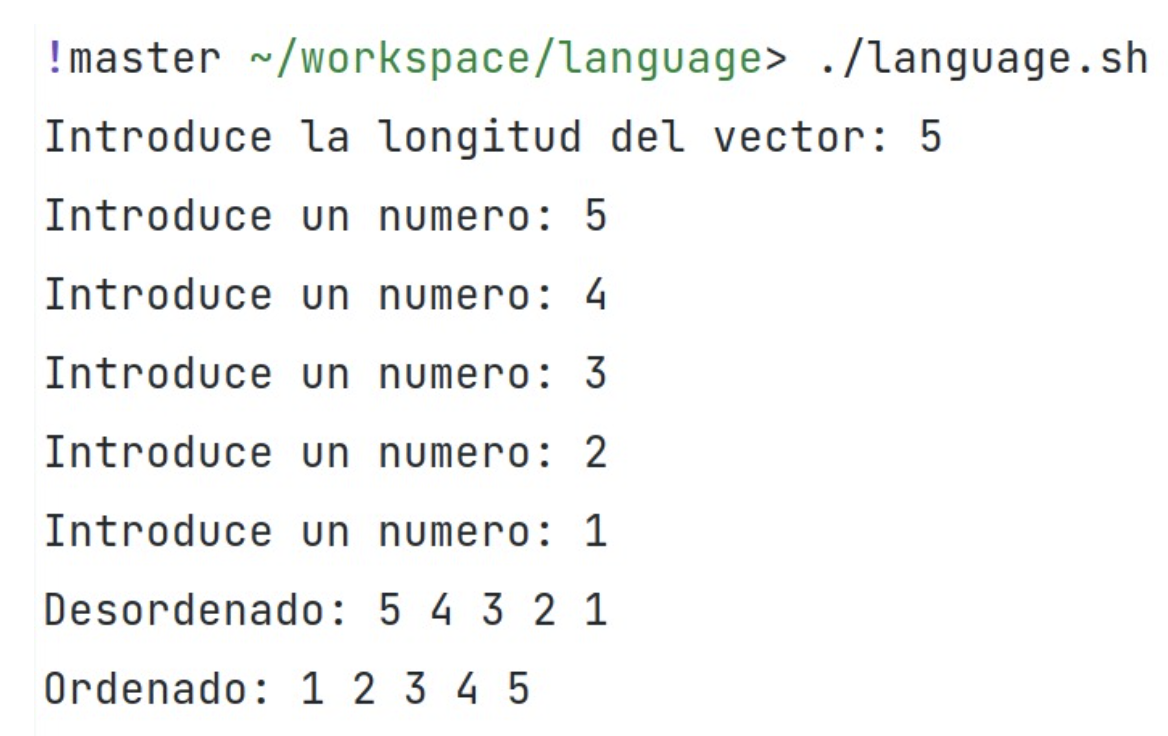
\includegraphics[width=\textwidth]{result.png}
        \end{figure}
    \end{frame}


    \section{Conclusiones}
    \begin{frame}{Conclusiones}
        \begin{itemize}
            \item Facilidad para la especificación formal de un lenguaje
            \item Facilidad para ejecutar el lenguaje
            \item Especificación de otros lenguajes de programación
            \item Verificación de propiedades
        \end{itemize}
    \end{frame}

    \section{Bibliografía}
    \begin{frame}{Bibliografía}
        \begin{itemize}
            \item Manual de maude \\
                    \url{http://maude.lcc.uma.es/maude31-manual-html/maude-manual.html}
            \item Maude como marco semántico ejecutable \\
            Alberto Verdejo \\
                    \url{http://maude.sip.ucm.es/alberto-verdejo/tesis/index.html}
            \item Formal Analysis of Java Programs in JavaFAN \\
            Azadeh FarzanFeng ChenJosé MeseguerGrigore Roşu \\
                \url{https://link.springer.com/chapter/10.1007/978-3-540-27813-9_46}
        \end{itemize}
    \end{frame}
\end{document}